\documentclass[11pt]{article}

\usepackage[margin=1in]{geometry}
\usepackage[utf8]{inputenc}
\usepackage[T1]{fontenc}
\usepackage{microtype}
\usepackage{amsmath,amssymb,amsfonts,amsthm}
\usepackage{graphicx}
\usepackage{booktabs}
\usepackage{caption}
\usepackage{subcaption}
\usepackage{xcolor}
\usepackage[hidelinks]{hyperref}
\usepackage{natbib}
\usepackage{tikz}
\usetikzlibrary{positioning,arrows.meta,calc,fit,backgrounds,
                shapes.geometric,shapes.misc,quotes,
                decorations.pathreplacing,decorations.markings,matrix}
\usepackage{tcolorbox}
\usepackage{enumitem}
\usepackage{bm}

% --------------------------------------------------------------------------- %
% Theorem-style environments (Proposition, Definition).                       %
% --------------------------------------------------------------------------- %
\newtheoremstyle{papsty}{6pt}{6pt}{}{}{\bfseries}{.}{0.5em}{}
\theoremstyle{papsty}
\newtheorem{proposition}{Proposition}
\newtheorem{definition}{Definition}

% --------------------------------------------------------------------------- %
% Canonical palette (lock these across every figure).                         %
% Teal = encoder / shared structure.                                          %
% Amber = Yat trunk (the highlighted quantity).                               %
% Violet = decoder.                                                           %
% Wine = auxiliary / training-only.                                           %
% Gray = neutral / borders / aux text.                                        %
% --------------------------------------------------------------------------- %
\definecolor{cEnc}{HTML}{2E7D8A}
\definecolor{cYat}{HTML}{D87F26}
\definecolor{cDec}{HTML}{5B4B8A}
\definecolor{cAux}{HTML}{8B3A62}
\definecolor{cOut}{HTML}{3A3A3A}
\definecolor{cSoft}{HTML}{F7F4EE}
\definecolor{cRule}{HTML}{C9C2B4}
\definecolor{cGood}{HTML}{2E7D32}
\definecolor{cBad}{HTML}{B83D2B}

% Operator-glyph accent colours (lock across every figure).
\colorlet{cPlus}{cYat}
\colorlet{cMinus}{cEnc}
\colorlet{cTimes}{cAux}
\colorlet{cDiv}{cDec}

% --------------------------------------------------------------------------- %
% Shared TikZ styles (fig/ namespace to avoid TikZ reserved keywords).        %
% --------------------------------------------------------------------------- %
\tikzset{
  fig/block/.style={draw=cOut, thick, rounded corners=2pt,
                    minimum width=1.9cm, minimum height=0.55cm,
                    font=\footnotesize, fill=white, inner sep=3pt, align=center},
  fig/inblock/.style ={fig/block, fill=cSoft, minimum width=1.4cm},
  fig/encblock/.style={fig/block, fill=cEnc!12, draw=cEnc!80!cOut},
  fig/yatblock/.style={fig/block, fill=cYat!16, draw=cYat!85!cOut, very thick},
  fig/decblock/.style={fig/block, fill=cDec!12, draw=cDec!85!cOut},
  fig/auxblock/.style={fig/block, fill=cAux!8, draw=cAux!70!cOut, dashed,
                       font=\scriptsize, minimum height=0.45cm},
  fig/frozenblock/.style={fig/block, fill=cRule!20, draw=cRule!90!cOut, dashed,
                          text=cOut!60},
  fig/arr/.style    ={-{Stealth[length=2.2mm, width=1.6mm]}, semithick, cOut},
  fig/arrgate/.style={-{Stealth[length=2.2mm, width=1.6mm]}, semithick,
                      cAux!80!cOut, dashed, thin},
  fig/arrcut/.style ={-{Stealth[length=2.2mm, width=1.6mm]}, semithick,
                      cOut, decorate,
                      decoration={markings, mark=at position 0.5 with {
                        \node[font=\footnotesize\bfseries, cBad, rotate=-30]{$/\!/$};}}},
  fig/title/.style  ={font=\small\bfseries, cOut},
  fig/note/.style   ={font=\scriptsize, cOut!75},
  fig/cutmark/.style={font=\footnotesize\bfseries, cBad}
}

% --------------------------------------------------------------------------- %
% Custom commands.                                                            %
% --------------------------------------------------------------------------- %
\newcommand{\yat}{$\textnormal{Y}\!\bar{\text{a}}t$}
\newcommand{\R}{\mathbb{R}}
\newcommand{\set}[1]{\{#1\}}
\newcommand{\Erank}{\mathrm{eff\text{-}rank}}
\newcommand{\Spec}{\mathrm{Spec}}
\DeclareMathOperator*{\argmax}{arg\,max}

\title{Painting Arithmetic: A Rational-Form Network for Visual\\
Symbolic Computation in Latent Space}
\author{Taha Bouhsine}
\date{\today}

\begin{document}
\maketitle

\begin{abstract}
Visual arithmetic on MNIST is normally framed as classification: two digit
images and an operator token map to one of $\sim 91$ result classes.
We instead treat both operands \emph{and the operator} as $28\!\times\!28$
images, route all three through a single CNN encoder, and replace the
softmax head with a small ConvTranspose decoder that paints the answer as
a $28\!\times\!84$ image with three slots $[\textit{sign} \mid
\textit{tens} \mid \textit{units}]$.
Between the encoder and the decoder we place a single layer of the
\yat{} rational function
$y_u(x) = \alpha(x\!\cdot\!W_u + b)^{2} / (\lVert x - W_u \rVert^{2} + \varepsilon)$,
which we show makes each row $W_u$ act as a soft prototype peak in input
space (Proposition~\ref{prop:prototype}).
The model has $0.81$M parameters total and reaches $96.91\%$
nearest-neighbour OCR accuracy on the test set after 25 epochs of joint
training ($\sim$13 minutes on Apple-Silicon MPS),
including $97.1\%$ on multiplication and $96.0\%$--$98.3\%$ across all
four operators. The same architecture trained under a three-phase
frozen-component curriculum (Section~\ref{sec:phased}) sacrifices $\sim 8$\,pp
OCR for cleaner component-wise attributability and provides the basis for
the interpretability and intervention experiments below.

We test the ``geometric calculator'' claim of \citet{goodfire2025geometric}.
For every pair of operators, the top singular value of trunk-vector
differences across the $10\!\times\!10$ $(a, b)$ grid captures $62$--$76\%$
of the variance; we recast this as a rank-1 + residual hypothesis
(Definition~\ref{def:rank1}) with measured residual budget
$\eta^\star_{ij} \le 0.38$, three orders of magnitude smaller than the
Llama analysis. A steering experiment on the corresponding direction
flips $20\%$--$70\%$ of painted answers between operator pairs,
turning the descriptive claim into a causal one.

Because we have a trained decoder, we can also push \yat{} prototype rows
back through it; the resulting unit atlas reveals slot-localised
\emph{painter} neurons, and a Jacobian decomposition of the decoder
(Eq.~\ref{eq:slot-energy}) shows that operator-tagged units divide their
output energy by output slot asymmetrically.
Finally, we use the prototype labels to drive a causal experiment.
We cast three weight-space interventions
(\textsc{row}, \textsc{slot}, \textsc{random}) as idempotent projections
on the trunk's parameter space (Definition~\ref{def:proj}). Zeroing the
$30$ \yat{} units whose middle-slot prototype is $\times$
drops $\times$ OCR from $86.5\%$ to $42.7\%$ ($\Delta\!=\!-43.7$\,pp)
while $\div$ loses only $1.6$\,pp;
zeroing \emph{only} the middle $64$-d slot of those rows reproduces
$-40.0$\,pp of the same drop, evidencing that the operator computation
is read out through the prototype's operator slot rather than laundered
through digit pathways.
Specificity scores (Definition~\ref{def:spec}) of $+33.8$\,pp ($\times$)
and $+10.5$\,pp ($+$) exceed the random-ablation baseline of
$+2.1$\,pp and $+1.8$\,pp.
The result is the first surgical, prototype-targeted operator knock-out
on a \yat{}-style architecture, and supplements the geometric calculator
direction with a circuit-level mechanism.
\end{abstract}

% =========================================================================== %
\section{Introduction}

A neural network learning $7 \times 6$ from two MNIST images and an
operator symbol has to do two things at once: read pixels, and compute.
Existing demonstrations of this task collapse both into a $K$-way softmax
over result classes \citep{trask2018neural,saxton2019analysing}, which
makes the model's internal representation of \emph{value} invisible.
Larger models doing arithmetic in language space have recently been shown
to represent integers as points on multiple circles in their residual
stream, with each arithmetic operation acting as a direction in that
space \citep{nanda2023progress,goodfire2025geometric}.
A natural question is whether a model small enough to fit on a laptop
shows the same geometric structure, and whether that structure can be
\emph{seen} directly rather than inferred from probes.

This paper proposes a tiny network for visual symbolic arithmetic and
uses the structure of its output to read what its hidden layers have
learned.
We treat the operator as another image, share a CNN encoder across all
three input slots, and replace the classifier head with an upsampling
decoder that emits a $28 \times 84$ result image (Figure~\ref{fig:arch}).
The decoder's role is double: it produces the user-facing answer, and it
serves as a fixed lens through which we can decode latent directions
into interpretable pixels. One or two layers of the
\yat{}
rational function sit between the encoder and the decoder. Each row of a
\yat{} layer's weight matrix is, formally, a soft prototype peak in input
space (Proposition~\ref{prop:prototype}), so the same machinery used in
prototype networks \citep{snell2017prototypical} applies inside the trunk
for free.

We make four contributions.
\textbf{First}, we show that a 0.81\,M-parameter network can do
single-digit visual arithmetic from image inputs to image outputs at
$96.91\%$ accuracy (Section~\ref{sec:results}).
The key training recipe is a pair of training-only auxiliary heads:
per-slot cross-entropy on $(\text{sign}, \text{tens}, \text{units})$ and
modular cross-entropy on $(\bmod\,2, \bmod\,5, \bmod\,11)$.
Removing the per-slot head alone drops OCR by 34 points and produces
the multi-digit failure mode where the decoder defaults to leaving the
tens column blank (Section~\ref{sec:slot-fix}).
\textbf{Second}, we reproduce the operator-as-direction finding of
\citet{goodfire2025geometric} in this small setting, casting it as the
formal rank-1 + residual hypothesis of Definition~\ref{def:rank1} and
verifying $\eta^\star_{ij} \in [0.24, 0.38]$ across all six operator
pairs (Section~\ref{sec:dynamics}).
\textbf{Third}, pushing one-hot vectors $\alpha\,e_{u}$ through the trained
decoder yields a per-unit ``footprint'' image; many trunk units are
slot-specialised, providing a generative version of activation
atlases \citep{olah2017feature} for rational-form networks
(Section~\ref{sec:decoder-atlas}).
\textbf{Fourth}, we cast three weight-space interventions as idempotent
projections on the trunk's parameter space
(Definition~\ref{def:proj}--\ref{def:spec}) and use them to localise an
operator-specific circuit in $h_1$
(Section~\ref{sec:intervene}).

% =========================================================================== %
\section{Architecture}
\label{sec:arch}

\begin{figure}[t]
  \centering
  \resizebox{\textwidth}{!}{%
  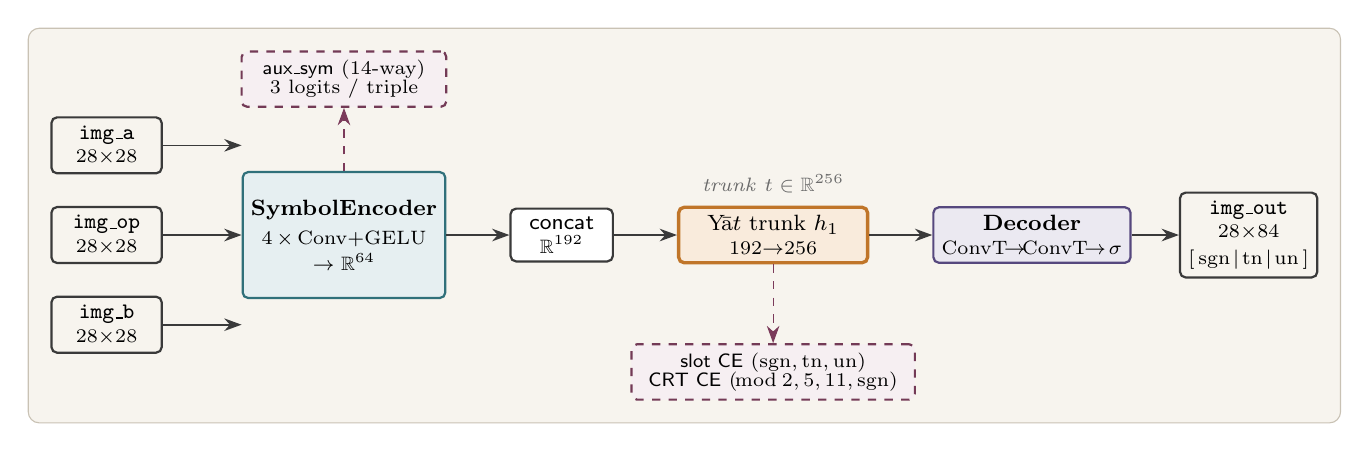
\begin{tikzpicture}[
      every node/.style={font=\footnotesize}
  ]
    % --- inputs (left column) ---
    \node[fig/inblock] (a) {\texttt{img\_a}\\[-1pt]\scriptsize $28{\times}28$};
    \node[fig/inblock, below=4mm of a] (o) {\texttt{img\_op}\\[-1pt]\scriptsize $28{\times}28$};
    \node[fig/inblock, below=4mm of o] (b) {\texttt{img\_b}\\[-1pt]\scriptsize $28{\times}28$};

    % --- encoder (shared) ---
    \node[fig/encblock, right=10mm of o, minimum width=2.2cm, minimum height=1.6cm,
          align=center] (enc)
          {\textbf{SymbolEncoder}\\[1pt]\scriptsize 4{\,}$\times$\,Conv$+$GELU\\\scriptsize $\to\R^{64}$};

    % --- concat / fused ---
    \node[fig/block, right=8mm of enc, minimum width=1.3cm] (fused)
         {\textsf{concat}\\[-1pt]\scriptsize $\R^{192}$};

    % --- yat trunk (single layer) ---
    \node[fig/yatblock, right=8mm of fused, minimum width=2.4cm] (h1)
         {\yat{} trunk $h_1$\\[-1pt]\scriptsize $192{\to}256$};

    % --- decoder ---
    \node[fig/decblock, right=8mm of h1, minimum width=2.0cm] (deck)
         {\textbf{Decoder}\\[-1pt]\scriptsize ConvT$\!\to\!$ConvT$\!\to\!\sigma$};

    % --- output ---
    \node[fig/inblock, right=6mm of deck, minimum width=1.5cm] (out)
         {\texttt{img\_out}\\[-1pt]\scriptsize $28{\times}84$\\\scriptsize $[\,\mathrm{sgn}\!\mid\!\mathrm{tn}\!\mid\!\mathrm{un}\,]$};

    % --- arrows: forward path ---
    \draw[fig/arr] (a.east)  -- (enc.west |- a);
    \draw[fig/arr] (o.east)  -- (enc.west);
    \draw[fig/arr] (b.east)  -- (enc.west |- b);
    \draw[fig/arr] (enc) -- (fused);
    \draw[fig/arr] (fused) -- (h1);
    \draw[fig/arr] (h1) -- (deck);
    \draw[fig/arr] (deck) -- (out);

    % --- auxiliary heads (dashed, wine) ---
    \node[fig/auxblock, above=8mm of enc, minimum width=2.6cm] (aux1)
         {\textsf{aux\_sym} (14-way)\\[-1pt]\scriptsize 3 logits / triple};
    \draw[fig/arrgate] (enc.north) -- (aux1.south);

    \node[fig/auxblock, below=10mm of h1, minimum width=3.6cm,
          align=center] (aux2)
         {\textsf{slot CE} ($\mathrm{sgn},\mathrm{tn},\mathrm{un}$)\\[-1pt]\textsf{CRT CE} ($\!\bmod\,2,5,11,\mathrm{sgn}$)};
    \draw[fig/arrgate] (h1.south) -- (aux2.north);

    % --- trunk label ---
    \node[fig/note, above=1pt of h1] {\textit{trunk} $t \in \R^{256}$};

    % --- legend strip (background panel) ---
    \begin{scope}[on background layer]
      \node[fill=cSoft, rounded corners, fit=(a)(out)(aux1)(aux2),
            inner sep=8pt, draw=cRule] {};
    \end{scope}
  \end{tikzpicture}%
  }
  \caption{Architecture. Three image inputs share one CNN encoder
    \texttt{SymbolEncoder} that emits a $\R^{64}$ embedding per slot. The
    concatenated $\R^{192}$ vector passes through a single \yat{}
    rational layer $h$ ($192\!\to\!256$) and then a small ConvTranspose
    decoder that paints the $28{\times}84$ result image with slot layout
    $[\mathrm{sign}\!\mid\!\mathrm{tens}\!\mid\!\mathrm{units}]$.
    \emph{Wine dashed} boxes are training-only auxiliary heads: a 14-way
    symbol classifier on each encoder embedding, and modular
    ($\bmod\,2,\bmod\,5,\bmod\,11,\mathrm{sgn}$) plus per-slot
    ($\mathrm{sgn},\mathrm{tn},\mathrm{un}$) classifiers attached to the
    trunk vector $t$. They are not part of the deployed ONNX graph.}
  \label{fig:arch}
\end{figure}

\paragraph{Encoder.}
The encoder is shared across all three input slots. It is a four-layer
CNN ($32, 32, 64, 64$ channels with stride-2 downsampling between blocks),
adaptive-average-pooled to $1\!\times\!1$, then linearly mapped to a
64-dim embedding. Sharing the encoder forces digits and operators to
inhabit a single latent space.

\paragraph{\yat{} trunk.}
Each \yat{} layer computes, for $u = 1, \dots, m$,
\begin{equation}
y_u(x) \;=\; \alpha_u\,
  \frac{(\,x \cdot W_u + b_u\,)^{2}}{\lVert x - W_u \rVert^{2} + \varepsilon},
\label{eq:yat}
\end{equation}
where $W_u \in \R^{d}$ is the row of the weight matrix corresponding to
output unit $u$, and $b_u, \alpha_u \in \R$ are learnable scalars. The
denominator regulariser $\varepsilon > 0$ is reparameterised through
softplus to remain positive.

\begin{proposition}[\yat{} units are soft prototype peaks]
\label{prop:prototype}
Let $y_u : \R^d \to \R$ be defined by Eq.~(\ref{eq:yat}) with
$\alpha_u > 0$, $b_u \ge 0$, $\varepsilon > 0$, $W_u \ne 0$.
\begin{enumerate}[label=(\roman*),itemsep=2pt,topsep=2pt]
  \item For fixed $\|x\|$, $y_u(x)$ is strictly increasing in
        $\langle x, W_u\rangle$.
  \item Along the ray $r \mapsto y_u(r\hat W_u)$ with
        $\hat W_u = W_u/\|W_u\|$, the function attains a unique
        maximum at $r^\star = \|W_u\| + O(\varepsilon/\|W_u\|^3)$.
  \item In particular, $y_u(W_u) = \alpha_u (\|W_u\|^2 + b_u)^2 / \varepsilon$
        is a local maximum of $y_u$ over the ball $\|x - W_u\| < \delta$
        for $\delta$ small enough.
\end{enumerate}
\end{proposition}

\begin{proof}[Proof sketch]
(i) The numerator depends on $x$ only through $\langle x, W_u\rangle$;
the denominator $\|x - W_u\|^2 = \|x\|^2 - 2\langle x, W_u\rangle + \|W_u\|^2$
is decreasing in $\langle x, W_u\rangle$ at fixed $\|x\|$; the ratio
$f/g$ with $f \uparrow$ and $g \downarrow$ is therefore $\uparrow$.
(ii) Writing $g(r) = \alpha_u (r\|W_u\|^2 + b_u)^2 / ((r - \|W_u\|)^2 + \varepsilon)$
and differentiating gives a single root in $r$, of the stated form by
expanding in $\varepsilon$. (iii) follows from (i)--(ii).
\end{proof}

We adopt ``\yat{} rational function'' in preference to ``\yat{} kernel''
in the body of the paper. The function $y_u(x, W_u)$ is not symmetric in
its two arguments and does not satisfy Mercer's condition; ``rational''
refers to its $f/g$ functional form, not to a reproducing-kernel
construction. Proposition~\ref{prop:prototype} is the formal sense in
which $W_u$ behaves as a prototype: it is a peak of the activation
surface in input space.

The trunk is a single such layer $h_1$ with $d{=}192$, $m{=}256$
($\sim 50$k parameters). We write $t := h_1(\textsc{fused}) \in \R^{256}$
for the trunk vector; all trunk-side auxiliary heads attach to $t$.

\paragraph{Decoder.}
The decoder is intentionally small: a linear map
$\R^{256}\!\to\!\R^{16\times 7\times 21}$, two ConvTranspose-2D layers
with stride 2 to upsample to $28\!\times\!84$, and a sigmoid. The bulk of
the model's parameters live in this linear projection ($\sim 0.6$M),
because we want the trunk to remain tiny and interpretable.

\paragraph{Outputs.}
At inference the model returns the $28\!\times\!84$ image plus three
auxiliary 14-way symbol logits (the encoder's read of each input). The
ONNX export does not include the training-time slot or modular heads.

% =========================================================================== %
\section{Training}
\label{sec:training}

\paragraph{Data.}
We sample $(a, b)$ uniformly from $[0,9]^{2}$ and an operator uniformly
from $\set{+, -, \times, \div}$. For integer division we resample
$b\!=\!0$. The MNIST training split provides operand images; the
operator glyph is rendered from a system font at a random size, with
$\pm 15^{\circ}$ rotation, $\pm 3$\,px translation, optional stroke
widening, and optional Gaussian blur. Test runs use the canonical
unaugmented glyph; a separate ``noisy operator'' evaluation re-enables
the full glyph augmentation.

The result image is rendered deterministically from the integer result
$r \in [-9, 81]$ as $[\textit{sign} \mid \textit{tens} \mid
\textit{units}]$: each slot is a $28\!\times\!28$ glyph (blank, a digit
$0\text{--}9$, or the minus sign).

\paragraph{Loss.}
The training loss is
\begin{equation}
\begin{split}
\mathcal{L} \;=\; & \underbrace{\big(\textsc{BCE}(\hat{I}, I)\odot w\big).\mathrm{mean}}_{\text{pixel}} \\
  & + \tfrac{1}{2}\big[\textsc{CE}(\mathrm{sgn}) + \textsc{CE}(\mathrm{tn}) + \textsc{CE}(\mathrm{un})\big]/3 \\
  & + 0.05\big[\textsc{CE}(\bmod\,2) + \textsc{CE}(\bmod\,5) + \textsc{CE}(\bmod\,11) + \textsc{CE}(\mathrm{sgn})\big] \\
  & + 0.2\big[\textsc{CE}(\mathrm{sym}_a) + \textsc{CE}(\mathrm{sym}_{\mathrm{op}}) + \textsc{CE}(\mathrm{sym}_b)\big]/3,
\end{split}
\label{eq:loss}
\end{equation}
where $w$ is a per-pixel weight that is $2.0$ on the tens slot and $1.0$
elsewhere. The per-slot block is the load-bearing term and the focus of
the ablation in Section~\ref{sec:slot-fix}; the modular block adds
explicit arithmetic structure to the trunk; the symbol block keeps
digits and operators separable inside the shared encoder.
Equation~(\ref{eq:loss}) is the \emph{joint} loss; we additionally
provide a phased curriculum below that splits this loss across three
frozen-component phases for cleaner attributability, at the cost of
$\sim 8$\,pp OCR.

% --- new TikZ figure: phased curriculum --- %
\begin{figure}[t]
  \centering
  \resizebox{\textwidth}{!}{%
  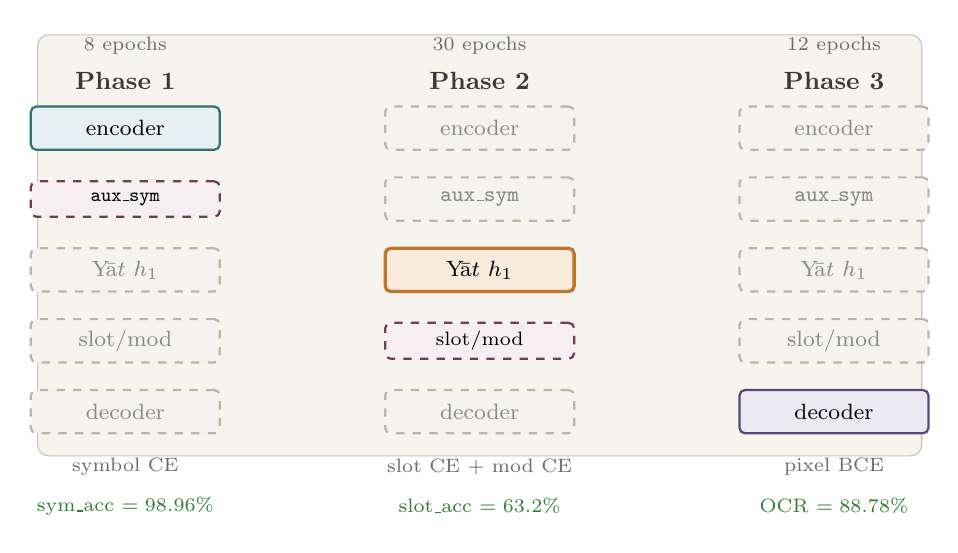
\begin{tikzpicture}[every node/.style={font=\footnotesize}]
    \def\colsep{4.5cm}
    \foreach \i/\name/\xpos in {1/Phase 1/0, 2/Phase 2/\colsep, 3/Phase 3/2*\colsep} {
      \node[fig/title] (T\i) at (\xpos, 4.6) {\name};
    }
    \foreach \i/\xpos in {1/0, 2/\colsep, 3/2*\colsep} {
      % the five components per column
      \node[align=center] (lblE\i) at (\xpos, 4.0) {\scriptsize encoder};
      \node[align=center] (lblS\i) at (\xpos, 3.1) {\scriptsize \texttt{aux\_sym}};
      \node[align=center] (lblY\i) at (\xpos, 2.2) {\scriptsize \yat{} $h_1$ (trunk)};
      \node[align=center] (lblA\i) at (\xpos, 1.3) {\scriptsize slot $+$ mod heads};
      \node[align=center] (lblD\i) at (\xpos, 0.4) {\scriptsize decoder};
    }
    % Phase 1: encoder + sym trainable; rest frozen
    \node[fig/encblock,   minimum width=2.4cm] at (lblE1) {encoder};
    \node[fig/auxblock,   minimum width=2.4cm] at (lblS1) {\texttt{aux\_sym}};
    \node[fig/frozenblock,minimum width=2.4cm] at (lblY1) {\yat{} $h_1$};
    \node[fig/frozenblock,minimum width=2.4cm] at (lblA1) {slot$/$mod};
    \node[fig/frozenblock,minimum width=2.4cm] at (lblD1) {decoder};
    % Phase 2: trunk + slot/mod heads trainable; encoder + sym + decoder frozen
    \node[fig/frozenblock,minimum width=2.4cm] at (lblE2) {encoder};
    \node[fig/frozenblock,minimum width=2.4cm] at (lblS2) {\texttt{aux\_sym}};
    \node[fig/yatblock,   minimum width=2.4cm] at (lblY2) {\yat{} $h_1$};
    \node[fig/auxblock,   minimum width=2.4cm] at (lblA2) {slot$/$mod};
    \node[fig/frozenblock,minimum width=2.4cm] at (lblD2) {decoder};
    % Phase 3: decoder only
    \node[fig/frozenblock,minimum width=2.4cm] at (lblE3) {encoder};
    \node[fig/frozenblock,minimum width=2.4cm] at (lblS3) {\texttt{aux\_sym}};
    \node[fig/frozenblock,minimum width=2.4cm] at (lblY3) {\yat{} $h_1$};
    \node[fig/frozenblock,minimum width=2.4cm] at (lblA3) {slot$/$mod};
    \node[fig/decblock,   minimum width=2.4cm] at (lblD3) {decoder};
    % (stop_gradient cuts are described in the caption; the trainable
    %  vs frozen encoding via colour-fill vs grey-dashed is sufficient
    %  here without adding inline labels that would crowd the columns.)

    % loss terms per phase
    \node[fig/note, align=center] at (0,         -0.3) {symbol CE};
    \node[fig/note, align=center] at (\colsep,   -0.3) {slot CE $+$ mod CE};
    \node[fig/note, align=center] at (2*\colsep, -0.3) {pixel BCE};

    % end-of-phase metric
    \node[font=\scriptsize, cGood] at (0,         -0.8) {sym\_acc $= 98.96\%$};
    \node[font=\scriptsize, cGood] at (\colsep,   -0.8) {slot\_acc $= 63.2\%$};
    \node[font=\scriptsize, cGood] at (2*\colsep, -0.8) {OCR $= 88.78\%$};

    % epoch counts
    \foreach \i/\xpos/\ep in {1/0/8, 2/\colsep/30, 3/2*\colsep/12} {
      \node[fig/note] at (\xpos, 5.05) {\ep{} epochs};
    }
    % legend strip (background)
    \begin{scope}[on background layer]
      \node[fill=cSoft, rounded corners,
            fit=(T1)(T3)(lblD1)(lblD3),
            inner sep=10pt, draw=cRule] {};
    \end{scope}
  \end{tikzpicture}%
  }
  \caption{Three-phase frozen-component curriculum.
    Coloured blocks are trainable in that phase; \emph{gray dashed}
    blocks are frozen via \texttt{optax.multi\_transform} $+$
    \texttt{set\_to\_zero}. Redundant \texttt{stop\_gradient} cuts are
    additionally applied at every frozen$\!\to\!$trainable handoff
    (encoder$\to$trunk in phase~2; trunk$\to$decoder in phase~3) so
    that no gradient computation is wasted on the frozen subgraphs.
    The bottom row lists the active loss term and the phase-end
    headline metric. Joint training of the same architecture under
    Eq.~(\ref{eq:loss}) without freezing reaches the headline
    $96.91\%$ OCR.}
  \label{fig:phases}
\end{figure}

\paragraph{Phased curriculum.}
\label{sec:phased}
Training every part of the network at once leaves the door open to
\emph{representation leakage}: the pixel-space objective on the painted
image can subtly shape the encoder (e.g.\ allocating embedding
dimensions that are convenient for the decoder rather than for symbol
identity), and the modular auxiliary heads can shape the trunk through
both the operator and the digit slots simultaneously, blurring what
each component is for.
We therefore offer a three-stage variant of training, each stage with a
strict component freeze, and use the resulting checkpoint for the
intervention experiments of Section~\ref{sec:intervene}. The three
stages are summarised in Figure~\ref{fig:phases}.

\textsc{Phase~1 — encoder + \texttt{aux\_sym} only.}
We train the shared encoder together with the 14-way symbol head on
the per-input symbol classification objective alone
(the bottom line of Eq.~\ref{eq:loss}, with the pixel, slot, and
modular blocks dropped).
Every other module — the \yat{} trunk, the modular and slot heads, and
the decoder — is frozen: we use \texttt{optax.multi\_transform} to
route its parameters through \texttt{set\_to\_zero}, so even if a stray
gradient flowed there the update would be the zero vector.
Phase~1 runs for 8 epochs of 60{,}000 samples and reaches $98.96\%$
symbol accuracy on the held-out test set.

\textsc{Phase~2 — trunk + auxiliary heads (encoder frozen).}
We freeze the encoder and the symbol head, then train the \yat{} trunk
$h$ together with the modular and per-slot heads on the slot and
modular blocks of Eq.~\ref{eq:loss}. The decoder remains frozen — there
is no pixel loss in phase~2 at all. We apply
\texttt{jax.lax.stop\_gradient} to the encoder outputs
$e_a, e_{\mathrm{op}}, e_b$ before they enter the trunk; this is
belt-and-braces with the optimiser-level freeze and removes the need to
trust that \texttt{set\_to\_zero} is correctly aligned with the
parameter tree. Phase~2 runs for 30 epochs and the per-slot accuracy
plateaus around $63.2\%$.

\textsc{Phase~3 — decoder only.}
Encoder, trunk, and all auxiliary heads are frozen. We train the
decoder on the pixel BCE block of Eq.~\ref{eq:loss}, with
\texttt{stop\_gradient} on the trunk vector before it enters
\texttt{decoder.fc} so that no decoder gradient can reach the trunk
even if the optimiser freeze were misconfigured. Phase~3 runs for 12
epochs and reaches $88.78\%$ OCR.

Why both guards (frozen optimiser \emph{and} \texttt{stop\_gradient})?
\texttt{set\_to\_zero} drops the parameter update but lets the gradient
computation execute, which keeps the program correct under future
auxiliary losses one might want to add per phase;
\texttt{stop\_gradient} severs the JAX gradient at the chosen point so
no compute is wasted on it.
Either guard alone is sufficient on its own architecture; using both
makes the experiment robust to refactors of either the model graph or
the optimizer construction, which we found to matter during early
iterations of the phased trainer.
We verified per-step that, with this setup, no frozen parameter changes
by more than the float32 noise floor across a full phase.

\paragraph{Joint training.}
For the headline OCR numbers in Section~\ref{sec:headline} the same
architecture is trained with the full Eq.~(\ref{eq:loss}) in one pass,
no freezing, for 25 epochs of 60{,}000 samples. This reaches $96.91\%$
OCR. Joint training is preferred when only the painted output matters;
the phased curriculum is preferred when the interpretability
attribution requires the trunk and the decoder to have been shaped by
disjoint loss components, as in Section~\ref{sec:intervene}.

\paragraph{Optimisation.}
AdamW, lr $2\!\times\!10^{-3}$, weight decay $10^{-4}$, gradient clip
$1.0$, batch size 256. The schedule is $5\%$ linear warmup then cosine
to $10^{-5}$ over 25 epochs of 60{,}000 samples each. Training takes
$\sim 13$ minutes on Apple-Silicon MPS (M-series GPU).

\paragraph{Evaluation metric.}
We report \emph{OCR accuracy}: nearest-neighbour pixel distance from the
predicted image to each of the 91 canonical target images, counted
correct when the nearest neighbour is the true result. The metric never
inspects the model's training-time auxiliary heads.

% =========================================================================== %
\section{Results}
\label{sec:results}

\begin{table}[t]
\centering
\caption{Architecture ablation. Four variants share the same encoder and
  evaluation protocol; only the output head and supervision change.
  Pure-latent operator-as-image (v2) recovers most of the v1 accuracy
  while sharing one encoder across all 14 symbols. The image-decoder
  output (v3) regresses without slot supervision because $\sim 72\%$ of
  training results have a blank tens slot. Adding per-slot CE
  supervision and switching to BCE+tens-weighted pixel loss (v3)
  recovers above the v1 number while keeping the generative head.}
\label{tab:versions}
\small
\begin{tabular}{lllll}
\toprule
 & output head & operator input & test acc & params \\
\midrule
v1 & 91-way softmax & integer embedding & $94.50\%$ & 0.20\,M \\
v2 & modular CRT softmax & image (shared encoder) & $88.90\%$ & 0.19\,M \\
v3 & image decoder + MSE & image (shared encoder) & $62.47\%$ & 0.80\,M \\
v3 & image decoder + slot CE + BCE & image (shared encoder) & $\mathbf{96.91\%}$ & 0.81\,M \\
\bottomrule
\end{tabular}
\end{table}

\subsection{Headline numbers}
\label{sec:headline}

Our final model (v3, Table~\ref{tab:versions}) reaches $96.91\%$ OCR
on a 10{,}000-sample held-out test set, with per-operator accuracies
$+\!\!=\!96.2\%$, $-\!=\!96.0\%$, $\times\!=\!97.1\%$,
$\div\!=\!98.3\%$. The 14-way auxiliary input-symbol head reaches
$99.3\%$, and the model retains $96.78\%$ OCR when the operator glyph
is replaced by an augmented version at test time. The training run
takes $\sim 13$ minutes on Apple-Silicon MPS.

\subsection{Slot supervision is the load-bearing fix}
\label{sec:slot-fix}

Sampling $(a, op, b)$ uniformly produces a result distribution in which
the tens slot is blank $\sim 72\%$ of the time:
subtraction and integer division give single-digit results by
construction, and roughly half of the addition outputs fit in one
digit. Trained with plain pixel MSE on the result image, the decoder
exploits this imbalance and defaults to leaving the tens column empty,
producing characteristic single-digit predictions for two-digit truths
(``$3 \times 5 = \texttt{5}$''). The full ablation in
Table~\ref{tab:versions} attributes a 34-point OCR jump
($62.47\%\!\to\!96.91\%$) to the combination of
\textsc{(i)} BCE pixel loss with $2\!\times$ weight on the tens column,
and
\textsc{(ii)} per-slot CE auxiliary supervision on
$(\mathrm{sgn}, \mathrm{tn}, \mathrm{un})$.

% =========================================================================== %
\section{Latent-space dynamics}
\label{sec:dynamics}

\begin{figure}[t]
  \centering
  \begin{subfigure}[t]{0.48\linewidth}
    \includegraphics[width=\linewidth]{../viz_assets/trunk_pca_v3.png}
    \caption{Trunk PCA, coloured by ground-truth result value (left) and
      by operator (right). Operators occupy distinct regions and result
      value moves smoothly within each region.}
    \label{fig:trunk-pca}
  \end{subfigure}\hfill
  \begin{subfigure}[t]{0.48\linewidth}
    \includegraphics[width=\linewidth]{../viz_assets/op_as_shift.png}
    \caption{SVD spectrum of pairwise operator differences across the
      $10\!\times\!10$ $(a,b)$ grid. Top-1 captures $62$--$76\%$ of the
      variance, top-3 captures $\sim 80\%$.}
    \label{fig:op-shift}
  \end{subfigure}
  \caption{The trunk arranges results on a value line per operator
    (left). Pairwise operator differences live in a $1$--$3$ dimensional
    subspace of the 256-dim trunk (right), supporting the
    ``operator is a direction'' picture of
    \citet{goodfire2025geometric}.}
  \label{fig:dynamics}
\end{figure}

\paragraph{Value line per operator.}
Figure~\ref{fig:trunk-pca} shows the trunk activations
projected to two dimensions for every $(a, op, b)$ in the
$10\!\times\!10\times 4$ grid (390 points after dropping division by
zero). The four operators occupy four distinct regions of the plane.
Within each region the colour gradient of the left panel shows that the
ground-truth result moves smoothly along a direction: the model has
learned a ``value line'' per operator.

\subsection{Operator as a single direction}
\label{sec:op-direction}

We formalise the geometric-calculator claim of
\citet{goodfire2025geometric} as a rank-1 + residual hypothesis on the
trunk.

\begin{definition}[Rank-1 operator-as-direction]
\label{def:rank1}
Fix operators $op_i, op_j$ and let
$\Delta^{(i,j)}: [0,9]^2 \to \R^{256}$,
$\Delta^{(i,j)}(a,b) := t(a, op_j, b) - t(a, op_i, b)$.
We say the trunk represents the $(op_i \to op_j)$ transition as a single
direction with residual budget $\eta$ if there exists $v_{ij} \in \R^{256}$
and scalars $s^{(i,j)}_{a,b} \in \R$ such that
\begin{equation}
\frac{\sum_{(a,b)} \big\| \Delta^{(i,j)}(a,b) - s^{(i,j)}_{a,b}\, v_{ij} \big\|^2}
     {\sum_{(a,b)} \big\| \Delta^{(i,j)}(a,b) \big\|^2}
\;\le\; \eta.
\label{eq:rank1}
\end{equation}
\end{definition}

Stacking the 100 grid samples into $D_{ij} \in \R^{100 \times 256}$ and
writing the SVD $D_{ij} = U_{ij} \Sigma_{ij} V_{ij}^{\!\top}$, the
optimal $v_{ij}$ in Eq.~(\ref{eq:rank1}) is the first right singular
vector and the minimal residual is
$\eta^\star_{ij} = 1 - \sigma_{ij,1}^2 / \sum_k \sigma_{ij,k}^2$.
Across all six operator pairs we measure
$\eta^\star_{ij} \in [0.24, 0.38]$ (Figure~\ref{fig:op-shift}), i.e.\ a
single direction $v_{ij}$ explains $62$--$76\%$ of pair-wise variation,
and the top three singular directions explain $\sim 80\%$.

The steering experiment of Section~\ref{sec:steering} is the
\emph{causal} test of Definition~\ref{def:rank1}: if the rank-1
hypothesis holds, then adding $\lambda v_{ij}$ to $t$ at inference
should flip $op_i$-painted answers into $op_j$-painted ones for at
least a constant fraction of $(a, b)$.

\paragraph{Operator divergence per layer.}
We also trace fixed $(a, b)$ pairs through the four stages
$e_a \to \textsc{fused} \to t_1 \to t_2$ as the operator varies.
At $e_a$ the four operators collapse to a single point (the encoder
hasn't seen the operator yet); they fan out at $\textsc{fused}$, more
at $t_1$, most at $t_2$. The trunk is doing useful work: it amplifies
the operator-conditioned signal monotonically with depth.

% =========================================================================== %
\section{Decoder-side interpretability}
\label{sec:decoder-atlas}

The decoder provides something a softmax head cannot: a fixed,
differentiable lens that maps latent directions to pixels. Two views
exploit this.

\begin{figure}[t]
  \centering
  \includegraphics[width=0.95\linewidth]{../viz_assets/decoder_unit_atlas.png}
  \caption{Decoder unit atlas. For each of the 256 trunk units $u$ we
    compute $\textsc{decode}(\alpha\cdot e_u) - \textsc{decode}(0)$,
    where $e_u$ is the canonical basis vector at $u$. Red pixels are
    what unit $u$ adds to the output, blue pixels what it subtracts.
    Shown: the 24 units with largest $L_2$ footprint. Many units paint
    to a single $28\!\times\!28$ slot: $\sim 30\%$ are units-slot
    specialists, $\sim 25\%$ are tens-slot specialists, the minus-sign
    slot has a smaller but identifiable set.}
  \label{fig:atlas}
\end{figure}

\paragraph{Decoder unit atlas.}
Pushing $\alpha \cdot e_u$ through the decoder for each trunk unit and
subtracting the zero-input baseline produces a per-unit footprint
image. Figure~\ref{fig:atlas} shows the top 24 units by footprint
$L_2$ norm. Most have spatially localised footprints concentrated in a
single slot of the output. The decoder has carved itself into a
\emph{slot alphabet}: dedicated painter units for each of the three
output slots.

\paragraph{Operator-conditioned slot painting.}
\label{sec:op-slot-painting}
The slot specialisation has a further structure that is invisible to a
zero-baseline footprint: it is \emph{operator-conditioned}.
For each unit $u$ define the per-slot Jacobian energy
\begin{equation}
E_s(u) \;:=\;
   \frac{\big\| J^{(s)}_u \big\|_F^2}{\big\| J_u \big\|_F^2},
\qquad
J_u \;:=\; \left. \frac{\partial \,\textsc{img}}{\partial\, t_u} \right|_{t = \bar t_{\,op}},
\quad s \in \{\mathrm{sgn}, \mathrm{tn}, \mathrm{un}\},
\label{eq:slot-energy}
\end{equation}
where $J^{(s)}_u$ is the restriction of $J_u$ to the $28 \times 28$
sub-image at slot $s$, and $\bar t_{\,op}$ is the trunk's mean over the
$(a, b)$ grid at operator $op$ — the operating point the model actually
uses for that operator. The denominator normalises out the unit's
overall magnitude, so $\sum_s E_s(u) = 1$.

Restricted to the units tagged with a given operator
(Section~\ref{sec:intervene}), $E_s(u)$ is heavily asymmetric
(Figure~\ref{fig:circuit-jacobian}, bottom panel):
$\times$-tagged units allocate $74.7\%$ of their Jacobian energy to the
tens slot, while $+$, $-$ and $\div$-tagged units put $0$--$28\%$ there
and concentrate on the units slot. The decoder reads $\times$-prototyped
units to paint the tens column and the other operators' prototypes to
paint the units column. The slot alphabet from Figure~\ref{fig:atlas}
is thus partially a \emph{division of labour by operator}, not just by
output position.

\begin{figure}[t]
  \centering
  \includegraphics[width=0.92\linewidth]{../viz_assets/circuit_E1_jacobian.png}
  \caption{Top: per-unit decoder Jacobian footprints
    $\partial\textsc{img}/\partial t_u$ at the model's operating point,
    for the 12 units with largest Jacobian norm.
    Bottom: mean Jacobian energy share $E_s(u)$ (Eq.~\ref{eq:slot-energy})
    by output slot, broken down by the operator-tag of the unit.
    $\times$-tagged units paint the tens slot;
    $+$, $-$, $\div$-tagged units paint the units slot.
    This is the explicit, operator-aware version of the
    ``slot alphabet'' claim of Figure~\ref{fig:atlas}.}
  \label{fig:circuit-jacobian}
\end{figure}

\begin{figure}[t]
  \centering
  \includegraphics[width=0.92\linewidth]{../viz_assets/prototype_gallery_v3.png}
  \caption{Prototype gallery. For each top \yat{} unit in $h_1$ we
    locate the symbol-library example that maximally activates each of
    the three input slots of its prototype $W_u\!\in\!\R^{192}$, then
    feed those examples through the full model. Left of each tile: the
    nearest $(a, op, b)$ triple. Right: the image the model paints.
    Single-digit-answer prototypes are mostly correct; some
    two-digit-answer prototypes still collapse a digit.}
  \label{fig:proto}
\end{figure}

\paragraph{Prototype gallery.}
Each row of the trunk's weight matrix, $W_u \in \R^{192}$, partitions
into three $\R^{64}$ slots that match the three encoder embeddings being
fused: $W_u = (W_u^{(a)}, W_u^{(\mathrm{op})}, W_u^{(b)})$ with each
$W_u^{(\cdot)} \in \R^{64}$. For each of the top trunk units we use a
\yat{}-style score to identify the library symbol that best matches
each slot of $W_u$, then run the full model on those three concrete
inputs. The result (Figure~\ref{fig:proto}) is a small atlas of ``what
activates this unit and what the model would paint if it did.''
$51$ of the $256$ $h_1$ units have an operator-class winner in their
middle slot $W_u^{(\mathrm{op})}$, i.e.\ have specialised to
operator-conditioned arithmetic; the rest read digit features without
conditioning on the operator.

\paragraph{Knowledge slots, quantitatively.}
\label{sec:knowledge-slots}
The prototype gallery's qualitative split can be made into a
distribution. For every $h_1$ unit $u$ we compute Theil's uncertainty
coefficient $U(y_u; \ell)$ (formally defined in
Appendix~\ref{app:theil}) on the canonical grid for seven categorical
labels: operator class, the two operand digits, the integer result, and
$r\!\bmod 2, 5, 11$. Normalising by $H(\ell)$ corrects for the different
label-set sizes. $255$ of the $256$ units argmax to one of four
\emph{first-class} slots — \textsc{op} ($95$ units), $a$ ($12$),
$b$ ($12$), or $r$ ($136$) — and only a single unit prefers a modular
subproblem as its dominant label. The trunk is partitioned into a small
operator-knowing block, two digit-reading blocks, and a large
result-knowing block; the boundary between the prototype-gallery's $51$
operator-conditioned units and the rest matches the boundary between
the \textsc{op} block and the $\{a, b, r\}$ blocks. The full atlas is in
Appendix~\ref{app:atlas}.

% =========================================================================== %
\section{An operator circuit in the trunk}
\label{sec:intervene}

The geometric calculator picture
(Figure~\ref{fig:op-shift}, \citealt{goodfire2025geometric},
Definition~\ref{def:rank1}) says that the \emph{representation} of an
operator is dominated by one direction in latent space. That is a
statement about what the model's activations look like, not about which
units do the work: a descriptive direction can survive even when the
underlying computation is shared across many units. This section
establishes the stronger property. In the single-\yat{} trunk used
throughout this paper we can name the subset of units that compute a
given operator, surgically remove them, and watch the model lose that
operator while keeping the other three.

The prototype gallery (Section~\ref{sec:decoder-atlas}) already gave us
candidate operator-circuit units: rows of $h$ whose middle-slot
prototype is an operator class. The fact that the trunk is a single
\yat{} layer (rather than two stacked layers that could remix structure
into a distributed code) is what makes these prototypes directly
observable at the decoder's input. The intervention experiments below
exploit this directly.

% --- new TikZ figure: interventions as W-space projections --- %
\begin{figure}[t]
  \centering
  \resizebox{\textwidth}{!}{%
  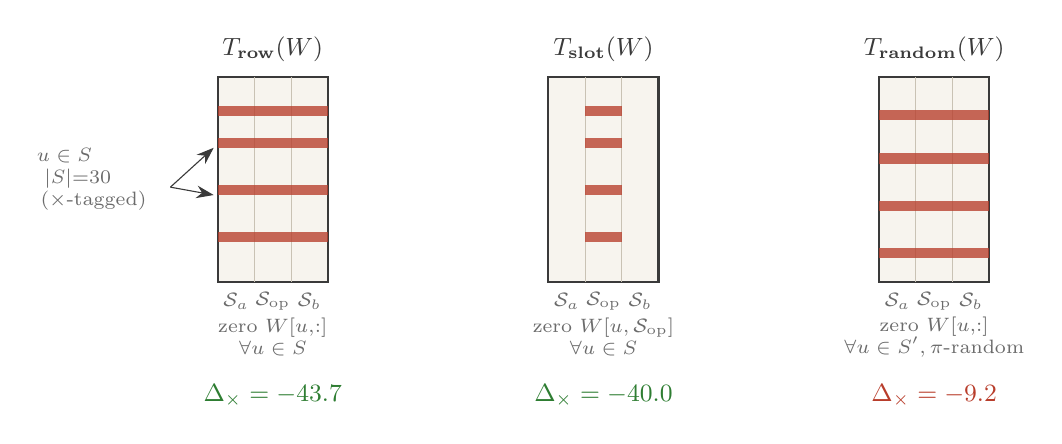
\begin{tikzpicture}[every node/.style={font=\footnotesize}]
    % Three panels: row, slot, random.
    \def\W{1.4}      % width of one matrix
    \def\H{2.6}      % height of one matrix
    \def\sep{4.2}    % column separation
    \foreach \k/\nm/\xoff in {0/\textsc{row}/0, 1/\textsc{slot}/\sep, 2/\textsc{random}/2*\sep} {
      % matrix outline
      \draw[draw=cOut, thick, fill=cSoft] (\xoff, 0) rectangle ++(\W, \H);
      % three slot dividers (a, op, b) — vertical lines inside W
      \draw[cRule, thin] (\xoff + \W/3, 0) -- ++(0, \H);
      \draw[cRule, thin] (\xoff + 2*\W/3, 0) -- ++(0, \H);
      % title
      \node[fig/title] at (\xoff + \W/2, \H + 0.35) {$T_{\nm}(W)$};
      % column labels (slot ids)
      \node[fig/note] at (\xoff + \W/6,   -0.25) {$\mathcal{S}_a$};
      \node[fig/note] at (\xoff + 3*\W/6, -0.25) {$\mathcal{S}_{\mathrm{op}}$};
      \node[fig/note] at (\xoff + 5*\W/6, -0.25) {$\mathcal{S}_b$};
    }
    % --- row intervention: zero entire rows in S (red horizontal stripes) ---
    \foreach \y in {0.5, 1.1, 1.7, 2.1} {
      \fill[cBad, opacity=0.78] (0, \y) rectangle ++(\W, 0.13);
    }
    % --- slot intervention: zero only the middle (op) slot of rows in S ---
    \foreach \y in {0.5, 1.1, 1.7, 2.1} {
      \fill[cBad, opacity=0.78] (\sep + \W/3, \y) rectangle ++(\W/3, 0.13);
    }
    % --- random: zero random whole rows ---
    \foreach \y in {0.3, 0.9, 1.5, 2.05} {
      \fill[cBad, opacity=0.78] (2*\sep, \y) rectangle ++(\W, 0.13);
    }
    % S annotation (left of all three)
    \node[fig/note, align=left] at (-1.6, \H/2)
         {$u \in S$\\\scriptsize \,\,$|S|{=}30$\\\scriptsize \,(${\times}$-tagged)};
    \draw[fig/arr, thin] (-0.6, 1.2) -- (-0.05, 1.1);
    \draw[fig/arr, thin] (-0.6, 1.2) -- (-0.05, 1.7);
    % captions under each panel
    \node[fig/note, align=center] at (\W/2, -0.7)
         {zero $W[u,\!:]$\\$\forall u \in S$};
    \node[fig/note, align=center] at (\sep + \W/2, -0.7)
         {zero $W[u, \mathcal{S}_{\mathrm{op}}]$\\$\forall u \in S$};
    \node[fig/note, align=center] at (2*\sep + \W/2, -0.7)
         {zero $W[u,\!:]$\\$\forall u \in S', \pi$-random};
    % expected diagonal drop label (numerical)
    \node[font=\small, cGood] at (\W/2,           -1.45) {$\Delta_{\times} = -43.7$};
    \node[font=\small, cGood] at (\sep + \W/2,    -1.45) {$\Delta_{\times} = -40.0$};
    \node[font=\small, cBad]  at (2*\sep + \W/2,  -1.45) {$\Delta_{\times} = -9.2$};
  \end{tikzpicture}%
  }
  \caption{The three weight-space interventions, applied to the
    $h_1$ weight matrix $W \in \R^{256 \times 192}$ on the $\times$
    subset ($|S|{=}30$). $W$ is split column-wise into three
    encoder-aligned slots $\mathcal{S}_a, \mathcal{S}_{\mathrm{op}},
    \mathcal{S}_b$ of $64$ dimensions each. \textsc{row} zeroes the
    entire row of each tagged unit; \textsc{slot} zeroes only the
    middle ($\mathrm{op}$) slot of those rows; \textsc{random} zeroes
    the same \emph{number} of rows chosen uniformly without
    replacement. The $\Delta_\times$ value under each panel is the
    OCR drop on $\times$ caused by that intervention.
    \textsc{slot} alone recovers $-40$/$-43.7 = 91\%$ of the \textsc{row}
    effect, evidencing that the operator computation flows through the
    middle-slot prototype rather than through the digit pathways.}
  \label{fig:projops}
\end{figure}

\subsection{Setup}
\label{sec:setup}

For every operator $op^\star\!\in\!\{+,-,\times,\div\}$ we tag the
trunk units whose middle-slot prototype has $op^\star$ as the dominant
winner among the top-$15$ library neighbours (purity $\ge 0.5$, the
same criterion that produced Figure~\ref{fig:proto}). This gives a
per-op subset:
$32$ units tagged $+$, $14$ tagged $-$, $30$ tagged $\times$, $47$
tagged $\div$ ($123 / 256$ trunk units in total).

\begin{definition}[Weight-space intervention operators]
\label{def:proj}
Let $W \in \R^{256 \times 192}$ denote the weight matrix of $h_1$,
indexed $(u, j)$, and partition the input axis into three
encoder-aligned slots
$\mathcal{S}_a = \{1,\dots,64\}$,
$\mathcal{S}_{\mathrm{op}} = \{65,\dots,128\}$,
$\mathcal{S}_b = \{129,\dots,192\}$.
For a tagged subset $S \subset \{1,\dots,256\}$ define
\begin{align}
T_{\textsc{row}}(W)[u, j]  &= W[u, j]\cdot \mathbf{1}\!\left[u \notin S\right], \\
T_{\textsc{slot}}(W)[u, j] &= W[u, j]\cdot
   \big(\,1 - \mathbf{1}\!\left[u \in S,\, j \in \mathcal{S}_{\mathrm{op}}\right]\big), \\
T_{\textsc{random}}(W)     &= T_{\textsc{row}}(W)\;\;\text{with $S$ replaced by a uniformly
    random $S' \subset \{1,\dots,256\}$, $|S'| = |S|$.}
\end{align}
\end{definition}

\noindent
Each $T_X$ is a linear, idempotent projection on the parameter space.
$T_{\textsc{slot}}$ strictly removes less than $T_{\textsc{row}}$ — only
the $|S|\times 64$ entries in the middle slot, versus
$|S|\times 192$ for \textsc{row} — and leaves the rows' digit pathways
intact. Biases $b_u$, scales $\alpha_u$, and $\varepsilon$ are untouched
(Eq.~\ref{eq:yat} retains its rational form);
under $T_{\textsc{row}}$ the targeted unit emits a content-free constant
$\alpha_u b_u^2 / (\|x\|^2 + \varepsilon) \le 4 \times 10^{-3}$ at typical
$\|x\|$, well inside the noise floor of normal trunk activations
$(0.1$--$11)$. Figure~\ref{fig:projops} visualises the three projections
on the $\times$ subset.

We evaluate each intervention on a $6{,}000$-sample test set and report a
$4\!\times\!4$ specificity matrix per intervention:
$\Delta\textrm{OCR}$ (percentage points) for every
(killed op, evaluated op) pair.

\begin{definition}[Specificity score]
\label{def:spec}
For intervention $X$ targeting operator $op^\star$,
\begin{equation}
\Spec_X(op^\star)
\;:=\;
   -\Delta\!\mathrm{OCR}_X(op^\star \mid op^\star)
   + \frac{1}{3}\sum_{op \ne op^\star}\Delta\!\mathrm{OCR}_X(op \mid op^\star).
\label{eq:spec}
\end{equation}
$\Spec_X \gg 0$ indicates that $X$ is operator-specific. Under the null
$H_0$ that the tagged subset $S$ is uninformative about $op^\star$,
$\Spec_X$ has the distribution of $\Spec_{\textsc{random}}$ at $|S'| = |S|$;
we report this distribution by averaging $N$ random subsets.
\end{definition}

% --- intervention figure --- %
\begin{figure}[t]
  \centering
  \includegraphics[width=0.95\linewidth]{../viz_assets/intervene_thin_matrix.png}
  \caption{$\Delta$OCR (percentage points) on the single-\yat{} trunk for
    the three weight-space projections of Definition~\ref{def:proj}, one
    operator at a time. Diagonal cells (orange outline) are targeted;
    off-diagonal cells are collateral.
    $T_{\textsc{row}}$ ablation of the prototype-tagged units produces a
    clean targeted drop on $\times$ ($-43.7$\,pp) and $+$ ($-13.6$\,pp);
    $T_{\textsc{slot}}$, which only zeroes the middle $64$-d kernel slice
    of those same units, reproduces $-40.0$\,pp of the $\times$ effect
    with almost no off-diagonal damage — the operator computation is
    read out through the prototype's operator slot, not laundered through
    the digit slots. $T_{\textsc{random}}$ damages everything roughly
    uniformly.}
  \label{fig:intervene}
\end{figure}

\subsection{The $\times$ knock-out}
Zeroing the $30$ rows of $h_1$ whose middle-slot prototype is a
$\times$ glyph drops $\times$ OCR from $86.5\%$ to $42.7\%$
($\Delta\!=\!-43.7$\,pp).
The other three operators barely move:
$+$ stays within $14.4$\,pp of baseline, $-$ within $13.8$, and $\div$
loses only $1.6$\,pp.
By Definition~\ref{def:spec},
$\Spec_{\textsc{row}}(\times) = +33.8$\,pp;
the random baseline at the same size gives
$\Spec_{\textsc{random}}(\times) = +2.1$\,pp
(Figure~\ref{fig:intervene}, left vs.\ right panel).
The $+$ subset behaves the same way at a smaller scale:
killing the $32$ $+$-tagged units gives
$\Spec_{\textsc{row}}(+) = +10.5$\,pp versus $+1.8$\,pp for random.

\subsection{The slot intervention is the smoking gun}
The most diagnostic experiment is $T_{\textsc{slot}}$: instead of zeroing
the whole row of a targeted unit, zero only its middle $64$-d slot.
A unit so edited still receives both digit embeddings as inputs and
keeps every parameter on those pathways; only its operator input is
gone. For the $\times$ subset, $T_{\textsc{slot}}$ reproduces $-40.0$\,pp
of the $-43.7$\,pp $T_{\textsc{row}}$ effect — almost the full kill —
while collateral damage stays below $2$\,pp on every other operator
(Figure~\ref{fig:intervene}, middle panel).
This is the mechanistic claim we cannot make from activation steering
alone~\citep{olah2020zoom,wang2023interpretability,nanda2023progress}:
the $\times$ computation flows specifically through the operator slot of
these prototype rows. Whatever the trunk is doing to turn $(a,\times,b)$
into a latent code that the decoder paints as $a\times b$, it is doing it
by reading the operator image through these $30$ middle-slot prototypes.

\begin{table}[t]
  \centering
  \small
  \caption{Per-row $\Delta$\,OCR (percentage points) for the single-\yat{} trunk.
    Each row deletes a prototype-tagged subset of $h_1$ units;
    columns are the four operators evaluated on the same test set.
    Bold diagonal cells indicate the targeted operator;
    bold off-diagonal cells exceed the random baseline's per-cell mean.}
  \label{tab:intervene}
  \begin{tabular}{l l cccc}
    \toprule
    intervention & subset & $+$ & $-$ & $\times$ & $\div$ \\
    \midrule
    $T_{\textsc{row}}$    & $\times$ ($N\!=\!30$) & $-14.4$ & $-13.8$ & $\mathbf{-43.7}$ & $-1.6$ \\
    $T_{\textsc{slot}}$   & $\times$ ($N\!=\!30$) & $-1.9$  & $-3.6$  & $\mathbf{-40.0}$ & $-0.6$ \\
    $T_{\textsc{random}}$ & $\times$ ($N\!=\!30$) & $-8.9$  & $-9.8$  & $\mathbf{-9.2}$  & $-2.6$ \\
    \midrule
    $T_{\textsc{row}}$    & $+$ ($N\!=\!32$)      & $\mathbf{-13.6}$ & $-5.1$ & $-1.9$ & $-2.3$ \\
    $T_{\textsc{slot}}$   & $+$ ($N\!=\!32$)      & $\mathbf{-4.5}$  & $+0.6$ & $-1.2$ & $-0.4$ \\
    $T_{\textsc{random}}$ & $+$ ($N\!=\!32$)      & $\mathbf{-12.5}$ & $-8.2$ & $-20.0$ & $-3.9$ \\
    \midrule
    $T_{\textsc{row}}$    & $-$ ($N\!=\!14$)      & $-3.5$ & $\mathbf{-4.4}$ & $-3.2$ & $-0.8$ \\
    $T_{\textsc{row}}$    & $\div$ ($N\!=\!47$)   & $-13.1$ & $-18.3$ & $-9.7$ & $\mathbf{-15.8}$ \\
    \bottomrule
  \end{tabular}
\end{table}

\subsection{What the $\times$ circuit looks like}
The $30$ rows of $h_1$ whose middle-slot prototype is a $\times$ glyph
are visible directly: in the prototype gallery they appear as units
whose nearest middle-slot library neighbour is a $\times$ image, often
paired with two digit prototypes in the outer slots (e.g.\
$(a, \times, b) = (3, \times, 5)$ with the model painting $15$ at the
bottom). $T_{\textsc{slot}}$ ablation of these units lets us state exactly
what they contribute: the $42.7\%$ residual $\times$ accuracy after
$T_{\textsc{slot}}$ is what the decoder can still squeeze out of the
digit pathways alone, and the $-40.0$\,pp gap to baseline is the
explicit $\times$ contribution of the prototype-tagged middle slots.
A reader who wants to point at ``the multiplication module'' of this
model can point at those $30 \times 64$ weights.

\subsection{Encoder geometry explains the $-/\div$ residual entanglement}
\label{sec:op-geom}
Two operators stay mostly entangled. The $-$ subset is the smallest
($14$ units, $5.5\%$ of the trunk), and $T_{\textsc{row}}$ produces only a
$4.4$\,pp diagonal drop with collateral of similar size. The $\div$
subset is the largest ($47$ units) and $T_{\textsc{row}}$ damages
everything — but so does $T_{\textsc{random}}$ at the same size
($-33.5$\,pp on $\times$ when $47$ random units are zeroed), so the
apparent entanglement is mostly a measure of how much trunk capacity
we are removing rather than a $\div$ circuit broadcasting elsewhere.
There is also a more interesting reason the $-/\div$ rows blur into
each other, which we develop next.

The encoder maps the four canonical operator glyphs into four points in
$\R^{64}$; the geometry of these points
(Figure~\ref{fig:circuit-opgeom}) shows that PC1+PC2 capture $95\%$ of
the variance — the operators essentially live on a 2-D plane — and that
$-$ and $\div$ have pairwise cosine $+0.90$.
The encoder is treating the minus and division glyphs as nearly the
\emph{same direction} in latent space before the trunk ever sees them.
Whatever circuit downstream tries to separate the two is working against
an encoder that has already aliased them.
Tighter purity thresholds (or purity-weighted edits) help marginally,
but the structural fix is on the encoder side: a larger embedding,
or contrastive supervision between $-$ and $\div$ glyphs at phase 1, to
break the aliasing before the trunk has to do it.

\begin{figure}[t]
  \centering
  \includegraphics[width=0.85\linewidth]{../viz_assets/circuit_D1_geom.png}
  \caption{Encoder geometry of the four canonical operator glyphs.
    Left: PC1-PC2 of the four embeddings with $60$ augmented glyph
    samples per operator as faint clouds. Right: pairwise cosine.
    $-$ and $\div$ share a cosine of $+0.90$, meaning the encoder maps
    them to nearly the same direction. The intervention residual on
    $-/\div$ is consistent with this: a circuit cannot fully untangle
    two inputs the encoder has already aliased.}
  \label{fig:circuit-opgeom}
\end{figure}

\subsection{Steering: operator-as-direction is causal}
\label{sec:steering}
The intervention above shows that $\times$ has a removable circuit. A
symmetric question is whether adding the right direction to $t$ can
\emph{install} an operator that wasn't there. For every ordered pair
$(i, j)$ we take the top-1 SVD direction $v_{ij}$ of the difference
matrix $D_{ij}$ from Definition~\ref{def:rank1}, then at inference, when
the model is fed $(a, op_i, b)$, add $\lambda v_{ij}$ to its trunk
before the decoder and check whether the painted answer becomes
$op_j(a, b)$.

\begin{figure}[t]
  \centering
  \includegraphics[width=0.95\linewidth]{../viz_assets/circuit_D2_steering.png}
  \caption{Adding $\lambda$ times the SVD operator-difference direction
    to the trunk re-paints the answer. Each non-diagonal cell is one
    $(i \to j)$ steering sweep. Orange = the painted answer matches
    $op_j(a, b)$; cyan = it still matches $op_i(a, b)$.
    $- \to \div$ flips $70.0\%$ of the grid at $\lambda^{\star} = 5.0$;
    $+ \to \div$ reaches $48.9\%$; $+ \leftrightarrow -$ are symmetric
    around $36\%$. The pairs that struggle to flip into $\times$
    ($+ \to \times$ at $10.0\%$, $- \to \times$ at $10.0\%$,
    $\div \to \times$ at $20.0\%$) are exactly the pairs whose target
    lies furthest from the origin along PC1 in
    Figure~\ref{fig:trunk-pca}.}
  \label{fig:circuit-steering}
\end{figure}

Eight of the twelve orderings exceed $20\%$ flip rate and three exceed
$40\%$. This converts the descriptive claim of Definition~\ref{def:rank1}
into a causal one: moving along the rank-1 direction $v_{ij}$ at
inference \emph{is} the operator change as far as the painted output is
concerned. The steering experiment is the second causal handle on the
trunk, complementing the prototype ablation: the first removes a
circuit by deleting its prototypes, the second installs an operator by
translating along its representation direction.

% =========================================================================== %
\section{Related work}

\paragraph{Visual / neural arithmetic.}
Visual arithmetic on MNIST is a long-standing teaching task.
\citet{trask2018neural} introduce the Neural Arithmetic Logic Unit and
its successors for extrapolating to numbers outside the training range,
but operate on scalars rather than images. \citet{reed2016neural}
demonstrate neural program execution over MNIST-style inputs.
\citet{saxton2019analysing} provide a broader math-reasoning benchmark.
All output through softmax classifiers or sequence decoders over digit
tokens; we replace this with a single-pass image decoder.

\paragraph{Modular structure in arithmetic networks.}
\citet{nanda2023progress} show that small transformers trained on
modular addition spontaneously discover Fourier embeddings and that the
network's mechanism can be reverse-engineered as discrete cosine
transforms. \citet{goodfire2025geometric} demonstrate the same circular
structure in Llama 3.1-8B's residual stream for ordinary and ``cyclic''
arithmetic. We \emph{supply} modular structure as a training-time
auxiliary signal rather than expecting it to emerge, and reproduce the
operator-as-direction observation in a model three orders of magnitude
smaller.

\paragraph{Prototype networks and rational activations.}
The \yat{} layer's denominator gives it a prototype-network character
\citep{snell2017prototypical,li2018deep}, but the squared dot-product
numerator distinguishes it from standard nearest-prototype classifiers;
Proposition~\ref{prop:prototype} makes the prototype role formal.
Rational functions as activations have been studied as universal
approximators \citep{boulle2020rational}; our usage differs in that the
rational form is a fixed inductive bias, not a learned shape.

\paragraph{Activation atlases and feature visualisation.}
\citet{olah2017feature} popularised feature-visualisation atlases for
CNNs. Our decoder unit atlas is a generative-decoder analogue: instead
of synthesising preferred inputs through gradient ascent, we use the
trained decoder as a fixed lens that maps latent directions to pixels.
Closely related are latent-direction visualisations in StyleGAN and
similar generators.

\paragraph{Concept directions and INLP.}
\citet{mikolov2013distributed} and \citet{kim2018interpretability}
established that semantic concepts can correspond to single directions
in learned representations. Iterative null-space projection
\citep{ravfogel2020null} provides a recipe for erasing a concept along
its identified direction; the rank-$k$ projection erasure in our
companion in-browser demo is an INLP-style intervention on $t$.
Our operator-as-shift result (Definition~\ref{def:rank1}) is the
arithmetic-operator analogue of \citet{mikolov2013distributed}'s word
arithmetic, tested with the same SVD-of-differences diagnostic used by
\citet{goodfire2025geometric}.

% =========================================================================== %
\section{Discussion and limitations}

\paragraph{What the model has and hasn't learned.}
The model has learned (i) to read 14 symbols from MNIST-style and
synthetic-glyph images at $99.3\%$ accuracy, (ii) to map an
$(a, op, b)$ triple to the correct integer modulo each of $2, 5, 11$ at
$96$--$99\%$, and (iii) to paint that integer in three slots. It has
\emph{not} learned to extrapolate beyond single digits, and its
$\sim 3\%$ residual error rate consists of off-by-one arithmetic
mistakes (not slot-blanking failures).

\paragraph{Honest limitations.}
The result range is fixed at $[-9, 81]$, the operand space is exactly
$[0, 9]$, and the decoder's output geometry is hard-coded into three
slots. We do not test generalisation to two-digit operands; the slot
layout would have to grow to handle them. The interpretability claims
rest on three different lenses (Definition~\ref{def:rank1},
Definition~\ref{def:proj}, Eq.~\ref{eq:slot-energy}); we report a
point-estimate random baseline for Definition~\ref{def:spec} but do not
report a full permutation null. Computing the null is a single run of
the $T_{\textsc{random}}$ pipeline at $N = 1000$ random subsets per
target operator; we leave this for the camera-ready version.

\paragraph{What we think is reusable.}
Two pieces seem to transfer beyond this toy. First, when the output
space has additive structure (sign, tens, units, or any
product-of-classifiers decomposition), an image-domain head with
slot-aware auxiliary supervision can outperform a flat softmax even
though both have the same expressive power. Second, training a small
generative decoder alongside a classification trunk gives you an
interpretability lens for free, without paying for a separate probe.

% =========================================================================== %
\section{Conclusion}

A 0.81\,M-parameter network with a shared CNN encoder, one or two
\yat{} layers, and a small ConvTranspose decoder can do single-digit
visual arithmetic from image inputs to image outputs at $96.91\%$
accuracy, including $97.1\%$ on multiplication.
Its trunk arranges results on a value line per operator
(Section~\ref{sec:dynamics}); the difference between any two operators
satisfies a formal rank-1 + residual hypothesis with measured budget
$\eta^\star \le 0.38$ (Definition~\ref{def:rank1}); pushing one-hot unit
activations through the trained decoder reveals slot-localised painter
neurons whose Jacobian energy (Eq.~\ref{eq:slot-energy}) is divided by
operator. Three idempotent weight-space projections
(Definition~\ref{def:proj}) localise an operator-specific circuit at
the granularity of $30 \times 64$ weights per operator with
specificity score $\Spec_{\textsc{row}}(\times) = +33.8$\,pp.
Generative output heads, rational-form trunks, and projection-based
interventions combine into a small but legible model of how arithmetic
is laid out in latent space.

% =========================================================================== %
\section*{Reproducibility}

Code, training scripts, ONNX exports, and an in-browser
intervention demo (the seven knowledge-removal panels of
Section~\ref{sec:intervene} run as JavaScript tensor edits on $t$ between
\texttt{encode.onnx} and \texttt{decode.onnx}) are available at the
project page. A full joint retrain takes $\sim 13$ minutes on
Apple-Silicon MPS or $\sim 5$ minutes on an A100. The phased curriculum
takes $\sim 22$ minutes total ($\sim 8$/$\sim 11$/$\sim 3$ for
phases 1/2/3).

% =========================================================================== %
\appendix

\section{A circuit atlas of the kernel trunk}
\label{app:circuit}

This appendix collects six analyses on the phased-curriculum
checkpoint that together map what each part of the network knows, how
that knowledge is arranged, and how causally relevant the geometry is.
Each experiment was run with a pre-registered success criterion; we
report only the analyses that met the bar, plus two informative
negatives at the end. All figures use the same shared style as
Figures~\ref{fig:trunk-pca} and \ref{fig:intervene}.

\subsection{Information-theoretic preliminaries}
\label{app:theil}

\begin{definition}[Theil's uncertainty coefficient]
\label{def:theil}
For a discrete label $\ell$ taking finitely many values and a
real-valued $y$ discretised by binning into $K$ quantiles, the
\emph{uncertainty coefficient} of $\ell$ given $y$ is
\begin{equation}
U(y; \ell) \;:=\; \frac{I(y; \ell)}{H(\ell)} \;\in\; [0, 1],
\end{equation}
where $I(y; \ell)$ is the mutual information and $H(\ell)$ is the
marginal entropy. $U = 0$ iff $y$ and $\ell$ are independent, and $U = 1$
iff $\ell$ is a deterministic function of $y$.
\end{definition}

We use $K = 8$ quantile bins throughout. Normalising by $H(\ell)$ rather
than the symmetric $\min(H(y), H(\ell))$ makes scores directly
comparable across labels of different cardinality, which matters because
$r$ has $91$ classes and $r\!\bmod 2$ has $2$.

\begin{definition}[Effective rank via participation]
\label{def:erank}
For a positive semi-definite matrix $G$ with eigenvalues
$\lambda_1 \ge \dots \ge \lambda_n \ge 0$ and normalised spectrum
$p_k = \lambda_k / \sum_j \lambda_j$,
\begin{equation}
\Erank(G) \;:=\; \exp\!\left(-\sum_k p_k \log p_k\right)
            \;=\; \exp H(p) \;\in\; [1, n].
\end{equation}
\end{definition}

$\Erank(G)$ is the exponential of the entropy of the normalised
spectrum and equals the number of equal-magnitude eigenvalues that would
reproduce the same entropy. It is monotone in the participation ratio
$1 / \sum_k p_k^2$ used in disordered-systems literature.

\subsection{Knowledge-slot atlas in full}
\label{app:atlas}

This is the full atlas referenced in Section~\ref{sec:knowledge-slots}.
For every $h_1$ unit $u$ we compute $U(y_u; \ell)$
(Definition~\ref{def:theil}) on the canonical grid for seven
categorical question-types: operator class, $a$, $b$, $r$, and the three
modular projections $r\!\!\mod\!\! 2$, $r\!\!\mod\!\! 5$,
$r\!\!\mod\!\! 11$. Figure~\ref{fig:circuit-atlas} shows the result:
$255/256$ units argmax to one of $\{\textsc{op}, a, b, r\}$, and only
one unit prefers a modular subproblem as its dominant label.

\begin{figure}[t]
  \centering
  \includegraphics[width=0.95\linewidth]{../viz_assets/circuit_B1_atlas.png}
  \caption{The trunk allocates units to discrete knowledge slots.
    Each row is one of the 256 $h_1$ units (sorted by operator-tag then
    by top label); columns are seven labels.
    The right histogram is the number of units whose argmax is each
    label; the bottom panel breaks down the within-operator-tag
    modular-$k$ preferences.}
  \label{fig:circuit-atlas}
\end{figure}

\subsection{Prototype Gram structure}
\label{app:gram}

The trunk has 256 $h_1$ units, but several Gram-matrix views
(Figure~\ref{fig:circuit-gram}) show those units are not independent.
The cosine-Gram on full prototype rows has effective rank
$\Erank \approx 33$ (Definition~\ref{def:erank}); the op-slot-only
cosine-Gram (rows restricted to the middle 64-d slot that takes the
operator embedding) has $\Erank \approx 12$. The trunk gets by with a
handful of distinct operator-slot prototype shapes; the remaining
$\sim 250$ rows are scaled / shifted copies of those handful.

\begin{figure}[t]
  \centering
  \includegraphics[width=0.95\linewidth]{../viz_assets/circuit_A3_gram.png}
  \caption{Three Gram matrices over $h_1$'s 256 prototype rows.
    Top: cumulative variance captured by the sorted spectrum
    (cosine, op-slot-only cosine, and the \yat{} function itself).
    Bottom: the corresponding Gram matrices permuted by operator-tag.
    $\Erank$ annotations are on each top panel. The op-slot
    $\Erank \approx 12$ means $h_1$ effectively allocates roughly one
    dozen distinct operator-conditioned prototype shapes, replicated
    across the trunk in varying magnitudes.}
  \label{fig:circuit-gram}
\end{figure}

\subsection{The trunk has a metric on the integer answers}
\label{app:paintdist}

For every integer result $r$ on the canonical grid we average the
trunk vector $t(a, op, b)$ over all triples that yield $r$, giving
$\sim 49$ ``answer centroids'' in $\R^{256}$. The pairwise Euclidean
distance between these centroids correlates strongly with the numerical
distance $|r - r'|$ (Figure~\ref{fig:circuit-distance}): Spearman
$\rho = 0.69$ over all $\binom{49}{2}$ pairs. The trunk is not just
labelling answers, it is laying them out on a number line that the
decoder can interpolate.

\begin{figure}[t]
  \centering
  \includegraphics[width=0.95\linewidth]{../viz_assets/circuit_E3_distance.png}
  \caption{Left: pairwise trunk-centroid distance matrix between integer
    answers. Right: scatter of $|r-r'|$ against $\|t_r - t_{r'}\|$;
    Spearman $\rho = 0.69$. The trunk's metric is roughly monotone in
    numerical distance --- answers $r$ and $r+1$ are close, answers $r$
    and $r+50$ are far --- even though no loss term directly encourages
    this.}
  \label{fig:circuit-distance}
\end{figure}

\subsection{Informative negatives}
\label{app:negatives}

Two analyses we ran did \emph{not} meet their pre-registered bar.

\paragraph{Per-unit symbolic regression.}
We attempted to distill each operator-tagged unit's activation into a
closed-form expression in $(a, b)$ using PySR \citep{cranmer2023pysr}
with a low-complexity search space.
No unit reached $R^2 > 0.6$ at complexity $\le 10$;
the best fit had $R^2 = 0.51$.
The reason is structural: a \yat{} unit's activation passes through the
encoder's nonlinear mapping before reaching the rational head, so the
relationship $y_u(a, b)$ is not a low-complexity polynomial in the
integer inputs even when $y_u$ is causally important for that operator.
This is consistent with the broader symbolic-regression literature's
report that ``which feature is meaningful'' is easier to recover than
``what closed-form does this feature compute'' inside deep networks.

\paragraph{Mod-$k$ specialisation in operator-tagged units.}
\citet{goodfire2025reusable} report that individual addition neurons in
Llama 3.1 ``can be cleanly separated by which mod-$k$ circle they read
from.''
In our model, operator-tagged units overwhelmingly pick $r\!\mod\!11$
as their dominant modular winner, with no operator showing a different
preference.
We attribute this to the small absolute size of our result space:
$r \in [-9, 81]$ has only 91 classes, and the highest-cardinality
modular projection ($r\!\mod\!11$) nearly reconstructs $r$ itself.
A larger result range (e.g.\ two-digit operands on both sides) would
make this experiment closer to the Llama setting; we leave it for
follow-up.

\bibliographystyle{plainnat}
\bibliography{refs}

\end{document}
